\documentclass[12pt]{article}
\usepackage[T1]{fontenc}
\usepackage[light,math]{iwona}
\usepackage[latin1]{inputenc}
\usepackage{amsmath}
\usepackage{ulem}
\usepackage{mathtools}
\usepackage{xspace}
\usepackage{xstring}
\usepackage[english]{babel}
\usepackage[font=small,labelfont=bf]{caption}
\usepackage[centering,includeheadfoot,margin=2cm]{geometry}
\usepackage{tikz}
\usetikzlibrary{calc,shapes,arrows,automata,trees,shadows,decorations.pathmorphing,positioning,
shapes.misc,shapes.arrows,chains,matrix,scopes,decorations.pathmorphing,backgrounds}

\begin{document}
\title{CS375 WK7}
\author{Jason N Mansfield}
\maketitle
%tikz terminal
\tikzset{
  nonterminal/.style={
    % The shape:
    rounded rectangle,
    % The size:
    minimum size=6mm,
    % The border:
    very thick,
    draw=purple!70!black!50,         % 50% red and 50% black,
                                  % and that mixed with 50% white
    % The filling:
    top color=white,              % a shading that is white at the top...
    bottom color=purple!70!black!20, % and something else at the bottom
    % Font
    font=\itshape
  },
  terminal/.style={
    % The shape:
    diamond,
    minimum size=6mm,
    % The rest
    very thick,draw=black!50,
    top color=white,bottom color=orange!20,
    font=\ttfamily},
  skip loop/.style={to path={-- ++(0,#1) -| (\tikztotarget)}}
}


{
  \tikzset{terminal/.append style={text height=1.5ex,text depth=.25ex}}
  \tikzset{nonterminal/.append style={text height=1.5ex,text depth=.25ex}}
  \tikzset{point/.append style={text height=1.5ex,text depth=.25ex}}
}
%end of tikz terminal stuff
%begin tape stuff
\tikzset{
    tape node/.style={
        on chain,
        draw,
        inner sep=1pt,
        outer xsep=0pt,
        minimum height=0.2cm,
        minimum width=0.2cm,
        text depth=0pt,
        font=\tiny\tt

    }
}

\newcommand*\myblackbox[1]{%
    \node[
        tape node,
       blue!90
    ] {#1};
}

\newcommand*\mygraybox[1]{%
    \begin{pgfonlayer}{background}
        \node[
            tape node,
            gray!60
        ] {#1};
    \end{pgfonlayer}
}

%end tape stuff

\begin{figure}
\begin{center}
\caption{Q01: FA}
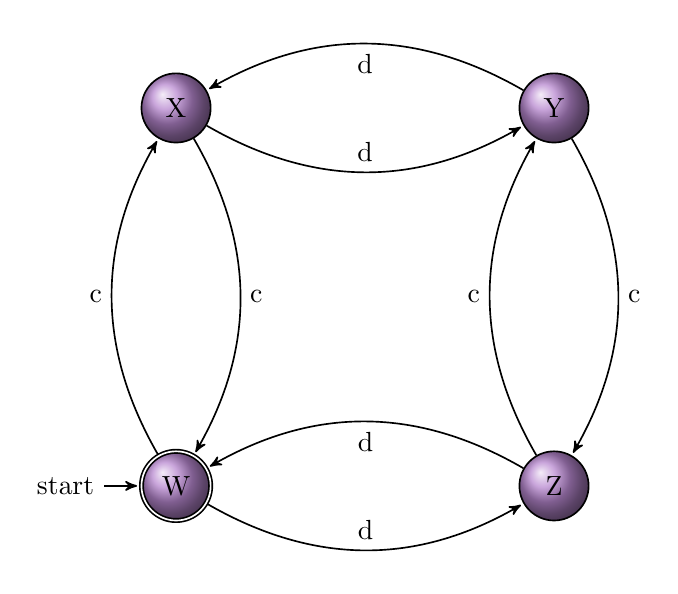
\begin{tikzpicture}[->,>=stealth',shorten >=1pt,auto,node distance=4.8cm, semithick]
\tikzstyle{every state}=[draw=black,text=black, ball color=red!40!blue!47!]
\node[state] (X) {X};
\node[state][right of=X](Y){Y};
\node[state,initial,accepting][below of=X](W){W};
\node[state][below of=Y](Z){Z};
\path (X)edge [bend right] node{d}(Y)
              edge [bend left] node{c}(W)
          (Y)edge [bend right]node{d}(X)
              edge [bend left]node{c}(Z)
          (W)edge [bend left]node{c}(X)
               edge[bend right]node{d}(Z)
          (Z)edge[bend left]node{c}(Y)
              edge[bend right]node{d}(W);      
\end{tikzpicture} 
\end{center}
\end{figure}


\begin{figure}
\begin{center}
\caption{Q01: PDA}
\begin{tikzpicture}[node distance=2.8cm,
        point/.style={coordinate},>=stealth',thick,draw=black!50,
        tip/.style={->,shorten >=0.007pt},every join/.style={rounded corners},
        hv path/.style={to path={-| (\tikztotarget)}},
        vh path/.style={to path={|- (\tikztotarget)}},
        text height=1.5ex,text depth=.25ex % align text horizontally
    ]
    %Standard Pushdown Symbols
   \node (start) [nonterminal]   {START};
   \node (accept) [nonterminal]   at (-3,-3.97)  {ACCEPT};
   \node (reject) [nonterminal]   at (9,-6.5) {REJECT};
   \node (reject2) [nonterminal]   at (-3,-6.5) {REJECT};
   %You will need multiple READ and POP Nodes with a varity of names.
   \node (W) [terminal,below=of start]                {READ};
   \node (X) [terminal,right=of W]                      {READ};
   \node (Y) [terminal,below=of X]                     {READ};
   \node (Z) [terminal,below=of W]                     {READ};
   \path (start)   edge[->] (W)  %  simple edges
             (W) edge[->]node[pos=0.50, above]{$\Delta$}(accept)
                   edge[->] node[pos=0.30, above]{c}(X)
                   edge[->] node[pos=0.30, left]{d}(Z);
   \path (X) edge[->] node[pos=0.30,right]{d}(Y);
   \draw [->]
     ( $ (X.north)$)    
     - ++(0,+1.1) 
    node[right]{c}
     -| ($(W.north)$);
  \draw [->]
     ( $ (Z.east)$) -++(1,0) node[right]{d} -++(1,4) -++(-.6,4);
  \draw [->]
     ( $ (Y.east)$) -++(1,0) node[right]{d} -++(1,4) -++(-.6,4);
   \draw [->]
     ( $ (Y.south)$) -++(0,-1) node[below]{c} -| ($(Z.south)$);
  \draw [->]
     ( $ (Z.south)$) -++(4.6,0) node[pos=0.30,above right]{c} ;
  \draw [->]
     ( $ (Z.south)$) -++(-3,0) node[pos=0.70,above right]{$\Delta$} -++(-3,2.7);
  \draw [->]
     ( $ (Y.south)$) -++(4.5,0) node[pos=0.70,above right]{$\Delta$} -++( 4.5,2.7);
 \draw [->]
     ( $ (X.east)$) -++(3.6,0) node[pos=0.70,above right]{$\Delta$} -++( 3.6,-2.2);
      
\end{tikzpicture}
\end{center}
\end{figure}
\clearpage

\begin{figure}
\begin{center}
\caption{Q02: FA}
\begin{tikzpicture}[->,>=stealth',shorten >=1pt,auto,node distance=4.8cm, semithick]
\tikzstyle{every state}=[draw=black,text=black, ball color=red!40!yellow!47!]
\node[state,accepting][right of=X](Y){Y};
\node[state][below of=X](W){W};
\node[state] (X)[below of=Y] {X};
\node[state,initial,accepting][above of=W](Z){Z};
\path (X)edge node{c}(Y)
              edge [loop right] node{d}(X)
          (Y)edge node{c}(W)
              edge [loop above]node{d}(Y)
          (W)edge node{c}(X)
               edge[loop left]node{d}(W)
          (Z)edge node{c}(W)
              edge node{d}(Y);      
\end{tikzpicture} 
\end{center}
\end{figure}

\begin{figure}
\begin{center}
\caption{Q02: PDA}
\begin{tikzpicture}[node distance=2.8cm,
        point/.style={coordinate},>=stealth',thick,draw=black!50,
        tip/.style={->,shorten >=0.007pt},every join/.style={rounded corners},
        hv path/.style={to path={-| (\tikztotarget)}},
        vh path/.style={to path={|- (\tikztotarget)}},
        text height=1.5ex,text depth=.25ex % align text horizontally
    ]
    %Standard Pushdown Symbols
   \node (start) [nonterminal]   {START};
   \node (accept) [nonterminal]   at (3.7,2)  {ACCEPT};
   \node (reject) [nonterminal]   at (2.5,-6.5) {REJECT};
   \node (push1) [nonterminal]   at (9,-8.5) {PUSH d};
   \node (push2) [nonterminal]   at (-3,-8.5) {PUSH d};
   \node (push3) [nonterminal]   at (9,-4) {PUSH d};
   %You will need multiple READ and POP Nodes with a varity of names.
   \node (Z) [terminal,below=of start]                {READ};
   \node (Y) [terminal,right=of Z]                      {READ};
   \node (W) [terminal,below=of Z]                    {READ};
   \node (X) [terminal,below=of Y]                     {READ};
   \node (pop1) [terminal]  at (7,-0.5)               {POP};
   \node (pop2) [terminal]  at (9,-2.3)               {POP};
   \node (pop3) [terminal]   at (3.7,0)                {POP};
   \draw [->] ( $ (Z.east)$) node[above]{d} -| ($(Y.west)$);
   \draw [->] ( $ (Z.south)$) node[left]{c} -| ($(W.north)$);
   \draw [->] ( $ (X.north)$) node[right]{c} -| ($(Y.south)$);
   \draw [->] ( $ (W.east)$) node[above]{c} -| ($(X.west)$);
   \draw [->] ( $ (Y.south)$) -++(-2,0) -++(-2,-1) node[pos=0.10,left]{c}-++(-4.6,-1);
   \draw [->] ( $ (Y.north)$) -++(0,1) -++(-2,1)node[above]{d} -++(-2,-0.9);
   \draw [->] ( $ (X.east)$) -++(2.5,0)node[pos=0.10,above]{d};
   \draw [->] ($(push3.south) $)-++(0,-1) node[pos=0.50,right]{d} -++(-4.3,-1) -| ($(Y.south)$);
   \draw [->] (push1.south) -++(0,-1) node[pos=0.50,right]{d} -++(-4.3,-1) -| ($(X.south)$);
   \draw [->] (push2.south) -++(0,-1) node[pos=0.50,right]{d} -++( 2.3,-1) -| ($(W.south)$);
   \draw [->] ($(W.west)$) node[above right]{d}  -| ($(push2.east)$) ;
   \draw [->] ($(Y.east)$) node[above right]{d}  -| ($(push3.west)$);
   \draw [->] ($(Y.east)$) -++(0,1) -| ($(pop2.west)$)node[pos=1,left]{d} ;
   \draw [->] ($(Y.east)$)  -++(0,1) -| ($(pop1.west)$)node[pos=.7,right]{c};
   \draw [->] (pop1.north) node[right]{c} -++(0,1.2);
   \draw [->] (pop2.north) -++(0,3) node[right]{d} --+(-4,3) --+(-4,-2);
   \draw [->] (Y.north) -++(0,2.5) node[pos=0.60,left]{$\Delta$} -++(-0.8,2.5);
   \path (W)[->]edge node[above]{$\Delta$}(reject);
   \path (X)[->]edge node[above]{$\Delta$}(reject);
   \path (start) [->]edge (Z);
   \path (Z) [->]edge node[above]{$\Delta$}(pop3);
   \path (pop3) [->]edge node[left]{$\Delta$}(accept);
    
\end{tikzpicture}
\end{center}
\end{figure}
\clearpage
\begin{figure}
\begin{center}
\caption{Q03a: Conversion Form}
\begin{tikzpicture}[node distance=2.8cm,
        point/.style={coordinate},>=stealth',thick,draw=black!50,
        tip/.style={->,shorten >=0.007pt},every join/.style={rounded corners},
        hv path/.style={to path={-| (\tikztotarget)}},
        vh path/.style={to path={|- (\tikztotarget)}},
        text height=1.5ex,text depth=.25ex % align text horizontally
    ]
    %Standard Pushdown Symbols
   \node (start) [nonterminal]   {START};
   \node (accept) [nonterminal] at (-5,-14.5)  {ACCEPT};
   \node (push1)[nonterminal] at (0,-4) {PUSH \$};
   \node (push2)[nonterminal] at (0,-10.5) {PUSH c};
   \node (push3)[nonterminal] at (0,-11.8) {PUSH c};
   \node (push4)[nonterminal] at (-3, -16.5) {PUSH c};
   \node (push5)[nonterminal] at (3, -16.5) {PUSH d};
   \node (push6)[nonterminal] at (-2.5,-10.5) {PUSH \$};
   \node (push7)[nonterminal] at (-2.5,-11.8) {PUSH c};
   %You will need multiple READ and POP Nodes with a varity of names.
   \node (pop1) [terminal]  at (0,-2)       {$POP_1$};
   \node (pop2) [terminal]  at (0,-8.5)    {$POP_2$};
   \node (pop7) [terminal]  at (-2.5,-8.5) {$POP_7$};
   \node (pop3) [terminal]  at (0,-16.5)  {$POP_3$};
   \node (pop4) [terminal]  at (-3,-19)   {$POP_4$};
   \node (pop5) [terminal]  at (3,-19)     {$POP_5$};
   \node (pop6) [terminal]  at (0,-22)     {$POP_6$};
   \node (pop8) [terminal] at (-5,-8.5)      {$POP_8$};
   \node (read1)[terminal] at (0,-6)        {$READ_1$};
   \node (read2)[terminal] at (0,-14)      {$READ_2$}; 
   \node (read3)[terminal] at (0,-19)      {$READ_3$};   
   %draw straight lines
   \draw [->] ( $ (start.south)$)  -| ($(pop1.north)$);
   \draw [->] ( $ (pop1.south)$) -|  ($(push1.north)$)node[above left]{\$};
   \draw [->] ( $ (push1.south)$)  -| ($(read1.north)$);
   \draw [->] ( $ (read1.south)$) -|  ($(pop2.north)$)node[right]{c};
   \draw [->] ( $ (read1.west)$) --+(-3,0) node[above]{$\Delta$}-|  ($(pop8.north)$);
   \draw [->] ( $ (pop2.south)$) -|  ($(push2.north)$)node[above left]{c};
   \draw [->] ( $ (push2.south)$) -|  ($(push3.north)$)node[above left]{c};
   \draw [->] ( $ (push3.south)$)  -| ($(read2.north)$);
   \draw [->] ( $ (read2.east)$)  --+(1,0) node[pos=0.60,above] {c} --+(1, 5)-| ($(pop2.east)$);
   \draw [->] ( $ (read2.south)$) -|  ($(pop3.north)$)node[right]{d};
   \draw [->] ( $ (pop3.south)$)  -| ($(read3.north)$)node[right]{c};
   \draw [->] ( $ (read3.west)$)  -| ($(pop4.east)$)node[above]{c};
   \draw [->] ( $ (read3.east)$)  -| ($(pop5.west)$)node[above]{d};
   \draw [->] ( $ (read3.south)$)  -| ($(pop6.north)$)node[left]{$\Delta$};
   \draw [->] ( $ (pop6.west)$) --+(-3,0) node[above]{$\$$}-| ($(accept.south)$);
   \draw [->] ( $ (pop4.north)$)  -| ($(push4.south)$)node[below left]{c};
   \draw [->] ( $ (pop5.north)$)  -| ($(push5.south)$)node[below right]{d};
   \draw [->] ( $ (push4.east)$)  -| ($(pop3.west)$);
   \draw [->] ( $ (push5.west)$)  -| ($(pop3.east)$);
   \draw [->] ( $ (read1.west)$) --+(-1,0) -|  ($(pop7.north)$)node[right]{$c$};
   \draw [->] ( $ (pop7.south)$) -|  ($(push6.north)$)node[above left]{\$};
   \draw [->] ( $ (push6.south)$) -|  ($(push7.north)$)node[above left]{c};
   \draw [->] ( $ (push7.south)$) --+(0,-1)-|  ($(read2.west)$);
   \draw [->] ( $ (pop8.south)$) -| node[left]{$\$$} ($(accept.north)$);
\end{tikzpicture}
\end{center}
\end{figure}
\clearpage
\begin{figure}
\begin{center}
\caption{Q03.a Summary Table}
\begin{tabular}{| l | c | c |c |c|c| }
\hline
FROM Where & To Where & READ What & POP What& PUSH What & ROW Number\\ \hline
START&$READ_1$&$\Lambda$&\$&\$&1\\ \hline
$READ_1$&ACCEPT&$\Lambda$&$\$$&-&2\\ \hline
$READ_1$&$READ_2$&c&\$&c\$&3\\ \hline
$READ_1$&$READ_2$&c&c&cc&4\\ \hline
$READ_2$&$READ_2$&c&c&cc&5\\ \hline
$READ_2$&$READ_3$&d&c&-&6\\ \hline
$READ_3$&$READ_3$&c&cc&c&7\\ \hline
$READ_3$&$READ_3$&d&dc&d&7\\ \hline
$READ_3$&$ACCEPT$&$\Lambda$&$\$$&-&8\\ \hline
\end{tabular}
\end{center}
\end{figure}
\begin{figure}
\begin{center}
\caption{Q03.a Productions}
Rule 1:
$S \rightarrow Net(START,ACCEPT,\$)$\\
Rule 2:\\
Net($READ_1$,ACCEPT,$\$$)$\rightarrow$ $Row_2$\\
Net($READ_2$,$READ_3$,$\$$)$\rightarrow$ $Row_6$\\
Net($READ_3$,ACCEPT,$\$$)$\rightarrow$ $Row_8$\\
Rule 3:\\
$Row_1 \rightarrow \Lambda$\\
$Row_2 \rightarrow \Lambda$\\
$Row_3 \rightarrow c$\\
$Row_4 \rightarrow c$\\
$Row_5 \rightarrow c$\\
$Row_6 \rightarrow d$\\
$Row_7 \rightarrow c$\\
$Row_8 \rightarrow c$\\
\end{center}
\end{figure}
%tape one
\DeclareRobustCommand*\drawboxes[1]{%
\begin{tikzpicture}[
        start chain=going right,
        node distance=0pt
    ]
    \IfSubStr{#1}{c1}{\myblackbox{c}}{\mygraybox{c}}%
    \IfSubStr{#1}{c2}{\myblackbox{c}}{\mygraybox{c}}%
    \IfSubStr{#1}{c3}{\myblackbox{c}}{\mygraybox{c}}%
    \IfSubStr{#1}{d1}{\myblackbox{d}}{\mygraybox{d}}%
    \IfSubStr{#1}{d2}{\myblackbox{d}}{\mygraybox{d}}%
    \IfSubStr{#1}{d3}{\myblackbox{d}~}{\mygraybox{d}~}
\end{tikzpicture}
}
%end tape one
\begin{figure}
\begin{center}
\caption{Q03.b}
\begin{tabular}{| l | c | r | }
\hline
STATE & STACK & TAPE\\ \hline
Start&$\Delta$&$\drawboxes{c1 c2 c3 d1 d2 d3} $\\ \hline
$Read_1$&$\Delta$&$\drawboxes{c2 c3 d1 d2 d3} $\\ \hline
Push&c$\Delta$&$\drawboxes{c2 c3 d1 d2 d3} $\\ \hline
$Read_2$&c$\Delta$&$\drawboxes{c3 d1 d2 d3} $\\ \hline
Push&cc$\Delta$&$\drawboxes{c3 d1 d2 d3} $\\ \hline
$Read_2$&cc$\Delta$&$\drawboxes{d1 d2 d3} $\\ \hline
Push&ccc$\Delta$&$\drawboxes{d1 d2 d3} $\\ \hline
$Read_2$&ccc$\Delta$&$\drawboxes{d2 d3} $\\ \hline
Pop&cc$\Delta$&$\drawboxes{d2 d3} $\\ \hline
$Read_3$&cc$\Delta$&$\drawboxes{d3} $\\ \hline
Pop&c$\Delta$&$\drawboxes{d3} $\\ \hline
$Read_3$&c$\Delta$&$\drawboxes{} $\\ \hline
Pop&$\Delta$&$\drawboxes{} $\\ \hline
$Read_3$&$\Delta$&$\drawboxes{} $\\ \hline
Pop&$\Delta$&$\drawboxes{} $\\ \hline
\textcolor{green!50!brown!89!}{Accept}&$\Delta$&$\drawboxes{} $\\ \hline
\end{tabular}
\end{center}
\end{figure}

%tape two
\DeclareRobustCommand*\drawboxes[1]{%
\begin{tikzpicture}[
        start chain=going right,
        node distance=0pt
    ]
    \IfSubStr{#1}{c1}{\myblackbox{c}}{\mygraybox{c}}%
    \IfSubStr{#1}{c2}{\myblackbox{c}}{\mygraybox{c}}%
    \IfSubStr{#1}{c3}{\myblackbox{c}}{\mygraybox{c}}%
    \IfSubStr{#1}{d1}{\myblackbox{d}}{\mygraybox{d}}%
    \IfSubStr{#1}{d2}{\myblackbox{c}}{\mygraybox{c}}%
    \IfSubStr{#1}{d3}{\myblackbox{d}~}{\mygraybox{d}~}
\end{tikzpicture}
}
%end tape two

\begin{figure}
\begin{center}
\caption{Q03.c}
\begin{tabular}{| l | c | r | }
\hline
STATE & STACK & TAPE\\ \hline
Start&$\Delta$&$\drawboxes{c1 c2 c3 d1 d2 d3} $\\ \hline
$Read_1$&$\Delta$&$\drawboxes{c2 c3 d1 d2 d3} $\\ \hline
Push&c$\Delta$&$\drawboxes{c2 c3 d1 d2 d3} $\\ \hline
$Read_2$&c$\Delta$&$\drawboxes{c3 d1 d2 d3} $\\ \hline
Push&cc$\Delta$&$\drawboxes{c3 d1 d2 d3} $\\ \hline
$Read_2$&cc$\Delta$&$\drawboxes{d1 d2 d3} $\\ \hline
Push&ccc$\Delta$&$\drawboxes{d1 d2 d3} $\\ \hline
$Read_2$&ccc$\Delta$&$\drawboxes{d2 d3} $\\ \hline
Pop&cc$\Delta$&$\drawboxes{d2 d3} $\\ \hline
$Read_3$&cc$\Delta$&$\drawboxes{d3} $\\ \hline
Pop&c$\Delta$&$\drawboxes{d3} $\\ \hline
$Read_3$&c$\Delta$&$\drawboxes{} $\\ \hline
Pop&$\Delta$&$\drawboxes{} $\\ \hline
$Read_3$&$\Delta$&$\drawboxes{} $\\ \hline
Pop&$\Delta$&$\drawboxes{} $\\ \hline
\textcolor{green!50!brown!89!}{Accept}&$\Delta$&$\drawboxes{} $\\ \hline
\end{tabular}
\end{center}
\end{figure}

%tape three
\DeclareRobustCommand*\drawboxes[1]{%
\begin{tikzpicture}[
        start chain=going right,
        node distance=0pt
    ]
    \IfSubStr{#1}{c1}{\myblackbox{c}}{\mygraybox{c}}%
    \IfSubStr{#1}{c2}{\myblackbox{c}}{\mygraybox{c}}%
    \IfSubStr{#1}{c3}{\myblackbox{c}}{\mygraybox{c}}%
    \IfSubStr{#1}{d1}{\myblackbox{d}}{\mygraybox{d}}%
    \IfSubStr{#1}{d2}{\myblackbox{c}}{\mygraybox{c}}%
    \IfSubStr{#1}{d3}{\myblackbox{c}~}{\mygraybox{c}~}
\end{tikzpicture}
}
%end tape three
\begin{figure}
\begin{center}
\caption{Q03.d}
\begin{tabular}{| l | c | r | }
\hline
STATE & STACK & TAPE\\ \hline
Start&$\Delta$&$\drawboxes{c1 c2 c3 d1 d2 d3} $\\ \hline
$Read_1$&$\Delta$&$\drawboxes{c2 c3 d1 d2 d3} $\\ \hline
Push&c$\Delta$&$\drawboxes{c2 c3 d1 d2 d3} $\\ \hline
$Read_2$&c$\Delta$&$\drawboxes{c3 d1 d2 d3} $\\ \hline
Push&cc$\Delta$&$\drawboxes{c3 d1 d2 d3} $\\ \hline
$Read_2$&cc$\Delta$&$\drawboxes{d1 d2 d3} $\\ \hline
Push&ccc$\Delta$&$\drawboxes{d1 d2 d3} $\\ \hline
$Read_2$&ccc$\Delta$&$\drawboxes{d2 d3} $\\ \hline
Pop&cc$\Delta$&$\drawboxes{d2 d3} $\\ \hline
$Read_3$&cc$\Delta$&$\drawboxes{d3} $\\ \hline
Pop&c$\Delta$&$\drawboxes{d3} $\\ \hline
$Read_3$&c$\Delta$&$\drawboxes{} $\\ \hline
Pop&$\Delta$&$\drawboxes{} $\\ \hline
$Read_3$&$\Delta$&$\drawboxes{} $\\ \hline
Pop&$\Delta$&$\drawboxes{} $\\ \hline
\textcolor{green!50!brown!89!}{Accept}&$\Delta$&$\drawboxes{} $\\ \hline
\end{tabular}
\end{center}
\end{figure}
%tape four
\DeclareRobustCommand*\drawboxes[1]{%
\begin{tikzpicture}[
        start chain=going right,
        node distance=0pt
    ]
    \IfSubStr{#1}{c1}{\myblackbox{c}}{\mygraybox{c}}%
    \IfSubStr{#1}{c2}{\myblackbox{c}}{\mygraybox{c}}%
    \IfSubStr{#1}{c3}{\myblackbox{c}}{\mygraybox{c}}%
    \IfSubStr{#1}{d1}{\myblackbox{c}}{\mygraybox{c}}%
    \IfSubStr{#1}{d2}{\myblackbox{d}}{\mygraybox{d}}%
    \IfSubStr{#1}{d3}{\myblackbox{d}~}{\mygraybox{d}~}
\end{tikzpicture}
}
%end tape four
\begin{figure}
\begin{center}
\caption{Q03.e}
\begin{tabular}{| l | c | r | }
\hline
STATE & STACK & TAPE\\ \hline
Start&$\Delta$&$\drawboxes{c1 c2 c3 d1 d2 d3} $\\ \hline
$Read_1$&$\Delta$&$\drawboxes{c2 c3 d1 d2 d3} $\\ \hline
Push&c$\Delta$&$\drawboxes{c2 c3 d1 d2 d3} $\\ \hline
$Read_2$&c$\Delta$&$\drawboxes{c3 d1 d2 d3} $\\ \hline
Push&cc$\Delta$&$\drawboxes{c3 d1 d2 d3} $\\ \hline
$Read_2$&cc$\Delta$&$\drawboxes{d1 d2 d3} $\\ \hline
Push&ccc$\Delta$&$\drawboxes{d1 d2 d3} $\\ \hline
$Read_2$&ccc$\Delta$&$\drawboxes{d2 d3} $\\ \hline
Push&cccc$\Delta$&$\drawboxes{d2 d3} $\\ \hline
$Read_2$&cccc$\Delta$&$\drawboxes{d3} $\\ \hline
Pop&ccc$\Delta$&$\drawboxes{d3} $\\ \hline
$Read_2$&ccc$\Delta$&$\drawboxes{} $\\ \hline
Pop&cc$\Delta$&$\drawboxes{} $\\ \hline
$Read_3$&cc$\Delta$&$\drawboxes{} $\\ \hline
Pop&c$\Delta$&$\drawboxes{} $\\ \hline
\textcolor{red}{Reject}&c$\Delta$&$\drawboxes{} $\\ \hline
\end{tabular}
\end{center}
\end{figure}
\clearpage
\begin{figure}
\begin{center}
\caption{Q05: Conversion Form}
\begin{tikzpicture}[node distance=2.8cm,
        point/.style={coordinate},>=stealth',thick,draw=black!50,
        tip/.style={->,shorten >=0.007pt},every join/.style={rounded corners},
        hv path/.style={to path={-| (\tikztotarget)}},
        vh path/.style={to path={|- (\tikztotarget)}},
        text height=1.5ex,text depth=.25ex % align text horizontally
    ]
    %Standard Pushdown Symbols
   \node (start) [nonterminal]   {START};
   \node (accept) [nonterminal]  at (-8,-16)       {ACCEPT};
   \node (push1)[nonterminal] at (0,-4) {PUSH \$};
   \node (push2)[nonterminal] at (-7, 0) {PUSH \$};
   \node (push3)[nonterminal] at (-7, -2) {PUSH a};
   \node (push4)[nonterminal] at (-7, -4) {PUSH b};
   \node (push5)[nonterminal] at (-7, -6) {PUSH \$};
    \node (push6)[nonterminal] at (-10, 0) {PUSH x};
   \node (push7)[nonterminal] at (-10, -2) {PUSH x};
   \node (push8)[nonterminal] at (-10, -4) {PUSH x};
   \node (push9)[nonterminal] at (-10, -6) {PUSH x};
   \node (push10) [nonterminal]  at (-2,-11)  {PUSH a};
   \node (push11) [nonterminal]  at ( 2,-11)  {PUSH b};
   %You will need multiple READ and POP Nodes with a varity of names.
   \node (pop1) [terminal]  at (0,-2)       {$POP_1$};
   \node (pop2) [terminal]  at (-4,0)       {$POP_2$};
   \node (pop3) [terminal]  at (-4,-2)       {$POP_3$};
   \node (pop4) [terminal]  at (-4,-4)       {$POP_4$};
   \node (pop5) [terminal]  at (-4,-6)       {$POP_5$};
   \node (pop6) [terminal]  at (-2,-9)       {$POP_6$};
   \node (pop7) [terminal]  at (2,-9)       {$POP_7$};
   \node (pop8) [terminal]  at (0,-13)       {$POP_8$};
   \node (pop9) [terminal]  at (-4,-16)       {$POP_9$};
   \node (read1)[terminal] at (0,-6)        {$READ_1$};
   \node (read2) [terminal]  at (0,-16)       {$READ_2$};
   %draw straight lines
   \draw [->] ( $ (start.south)$)  -| ($(pop1.north)$);
   \draw [->] ( $ (pop1.south)$) -|  ($(push1.north)$)node[above left]{\$};
   \draw [->] ( $ (push1.south)$)  -| ($(read1.north)$);
   \draw [->] ( $ (read1.west)$) -++(-0.8,0) -++(-0.8,6)-++(-1.9,6)node[above]{a};
   \draw [->] ( $ (read1.west)$) -++(-0.8,0) -++(-0.8,4)-++(-1.9,4)node[above]{a};
   \draw [->] ( $ (read1.west)$) -++(-0.8,0) -++(-0.8,2)-++(-1.9,2)node[above]{b};
   \draw [->] ( $ (read1.west)$) -++(-0.8,0) -++(-0.8,0)-++(-1.9,0)node[above]{b};
   \draw [->] ( $ (pop2.west)$)  -| ($(push2.east)$)node[above right]{\$};
   \draw [->] ( $ (pop3.west)$)  -| ($(push3.east)$)node[above right]{a};
   \draw [->] ( $ (pop4.west)$)  -| ($(push4.east)$)node[above right]{b};
   \draw [->] ( $ (pop5.west)$)  -| ($(push5.east)$)node[above right]{\$};
   \draw [->] ( $ (push2.west)$)  -| ($(push6.east)$);
   \draw [->] ( $ (push3.west)$)  -| ($(push7.east)$);
   \draw [->] ( $ (push4.west)$)  -| ($(push8.east)$);
   \draw [->] ( $ (push5.west)$)  -| ($(push9.east)$);
   \draw [->] ( $ (push9.west)$) -++(-0.8,0)-++(-0.8,7.5) -++( 9.5,7.5) -++(9.5,1.4) -++(10.89,1.4);
   \draw[->] ( $ (push8.west)$)-++(-0.8,0);
   \draw[->] ( $ (push7.west)$)-++(-0.8,0);
   \draw[->] ( $ (push6.west)$)-++(-0.8,0);
   
\end{tikzpicture}
\end{center}
\end{figure}
\clearpage


\end{document}